%% ============================================================
%%  Privacy-Preserving Federated IDS for IoV using
%%  Single-Key CKKS Homomorphic Encryption and ChebyshevKAN
%%
%%  IEEE Conference Paper — IEEEtran two-column format
%% ============================================================
\documentclass[conference]{IEEEtran}

%% ------ Packages -----------------------------------------------
\usepackage{cite}
\usepackage{amsmath,amssymb,amsfonts}
\usepackage{algorithmic}
\usepackage{algorithm}
\usepackage{graphicx}
\usepackage{textcomp}
\usepackage{xcolor}
\usepackage{booktabs}
\usepackage{multirow}
\usepackage{url}
\usepackage{pgfplots}
\pgfplotsset{compat=1.18}
\usepackage{tikz}
\usetikzlibrary{arrows.meta, positioning, shapes.geometric, fit, backgrounds}

%% ------ Metadata -----------------------------------------------
\def\BibTeX{{\rm B\kern-.05em{\sc i\kern-.025em b}\kern-.08em
    T\kern-.1667em\lower.7ex\hbox{E}\kern-.125emX}}

\begin{document}

%% ============================================================
%%  TITLE AND AUTHORS
%% ============================================================
\title{Privacy-Preserving Federated Intrusion Detection for\\
Internet of Vehicles Using Single-Key CKKS\\
Homomorphic Encryption and ChebyshevKAN}



\maketitle

%% ============================================================
%%  ABSTRACT
%% ============================================================
\begin{abstract}
Modern vehicular networks face escalating cyber threats, including
Controller Area Network (CAN) bus injection attacks and Vehicle-to-Everything
(V2X) misbehaviour. Federated Learning (FL) enables collaborative intrusion
detection without sharing raw vehicle telemetry, yet the aggregation server
remains an honest-but-curious adversary capable of inverting individual
model updates to reconstruct sensitive driving data. This paper proposes a
privacy-preserving federated Intrusion Detection System (IDS) for the Internet
of Vehicles (IoV) that combines Single-Key Cheon--Kim--Kim--Song (CKKS)
Homomorphic Encryption (HE) with a novel \emph{ChebyshevKAN} neural network
classifier. The CKKS scheme ($N{=}8192$, 128-bit Ring-LWE security, $2^{40}$
fixed-point scale) packs 4,096 encrypted real-valued parameters per ciphertext,
enabling the RSU server to aggregate 44,164-parameter model updates entirely
within the encrypted domain. By relying strictly on CKKS for payload confidentiality
and operating under a secure physical channel assumption, we eliminate legacy
AES-256 and TLS transport overhead, substantially easing onboard ECU computation.
Extensive experiments on four heterogeneous IoV datasets---Car-Hacking (CAN),
IEEE VTC-CAN, CICIDS-2017, and VeReMi---under a non-IID Dirichlet partition
($\alpha{=}0.3$, 10 clients, 5 rounds) demonstrate that CKKS encryption introduces
a maximum accuracy degradation of only $0.01$ percentage points (pp) relative
to plaintext federated averaging, with a per-client ciphertext overhead of
${\approx}3.6$ MB and $1.76$ s per aggregation round. The system guarantees that
individual client updates remain private throughout training, verified by a runtime
audit asserting zero individual-update decryptions across all rounds.
\end{abstract}

\begin{IEEEkeywords}
Internet of Vehicles, Federated Learning, Homomorphic Encryption, CKKS,
Intrusion Detection, CAN Bus, ChebyshevKAN, Privacy-Preserving Machine
Learning, Non-IID, Byzantine Robustness
\end{IEEEkeywords}

%% ============================================================
%%  I. INTRODUCTION
%% ============================================================
\section{Introduction}

Modern vehicles are embedded computing platforms: a single automobile
integrates over 100 Electronic Control Units (ECUs), communicates over the
Controller Area Network (CAN) bus internally, and exchanges safety-critical
V2X messages externally. This attack surface is substantial. Demonstrated
attacks include remote CAN injection that commands braking and steering
\cite{miller2015remote}, RPM spoofing, and Fuzzy frame injection, all
achievable without physical access.

\textbf{Collaborative IDS and the privacy dilemma.}
No single vehicle observes the full diversity of the attack landscape: one
vehicle on a highway encounters DoS flooding; another at an intersection sees
gear-spoofing. Pooling raw CAN logs to a central server would produce
far stronger detectors, but the logs encode location history, driving
behaviour, and vehicle identity---information that cannot leave the vehicle
without regulatory and commercial consequences.

Federated Learning \cite{mcmahan2017fl} solves the raw-data problem: vehicles
train locally and share only model updates. However, sharing gradient
vectors introduces a new threat: a semi-honest aggregation server can apply
gradient inversion attacks \cite{zhu2019deep} to reconstruct training
samples from individual updates. Even a Road-Side Unit (RSU) operated by an
infrastructure vendor is a potential adversary of this type.

\textbf{Homomorphic Encryption as the answer.}
Encrypting model updates under a Fully Homomorphic Encryption (FHE) scheme
allows the server to aggregate ciphertexts without ever decrypting them.
The Cheon--Kim--Kim--Song (CKKS) scheme \cite{ckks2017} is uniquely suited
to this task: it natively encodes vectors of approximate real numbers and
packs thousands of floating-point weights into a single ciphertext via SIMD
batch encoding---a decisive advantage over Paillier (one value per ciphertext)
or BFV/BGV (integer-only).

\textbf{The Byzantine robustness challenge.}
Blinding the server creates a new vulnerability: Byzantine poisoning attacks,
where malicious vehicles submit adversarial updates, are harder to detect
when the server cannot inspect individual updates. Our initial design
\cite{generation1report} employed Multi-Krum \cite{blanchard2017machine} and
TOPSIS \cite{hwang1981topsis} for robust aggregation---both require pairwise
plaintext distances and are therefore incompatible with HE. We adopt the
FheFL framework's non-poisoning-rate scoring \cite{fhefl2023}, which computes
the squared distance to the global model entirely in the encrypted domain.

\textbf{Contributions.} This paper makes the following contributions:
\begin{enumerate}
  \item A complete Single-Key CKKS federated IDS architecture for IoV, with
        a formal threat model focusing on honest-but-curious server blindness
        without redundant transport-layer encryption.
  \item \emph{ChebyshevKAN}: a 44,164-parameter Chebyshev-polynomial
        Kolmogorov--Arnold Network (KAN) \cite{liu2024kan} replacing both
        MLP and the larger MamKANformer backbone, achieving a $14\times$
        parameter reduction that directly reduces ciphertext count,
        V2X bandwidth, and aggregation latency.
  \item A unified 46-dimensional feature extractor mapping CAN bus,
        IP-flow, and V2X-kinematic data into one representation, enabling a
        single model to serve four heterogeneous datasets.
  \item Empirical results across Car-Hacking, VTC-CAN, CICIDS-2017 and
        VeReMi showing ${\le}0.01$ pp accuracy gap between CKKS and
        plaintext federation, with $3.12{\times}10^{-8}$ maximum parameter
        error from CKKS approximation.
\end{enumerate}

%% ============================================================
%%  II. RELATED WORK
%% ============================================================
\section{Related Work}

\textbf{Federated IDS for IoV.}
Early federated IDS proposals for vehicular networks \cite{li2020federated}
train collaborative classifiers over raw CAN features without privacy
guarantees. These systems assume an honest server and share gradient
updates in plaintext, leaving them vulnerable to gradient inversion
\cite{zhu2019deep} and model poisoning attacks.

\textbf{Homomorphic Encryption in Federated Learning.}
FATE \cite{fate2019} integrates Paillier HE for logistic regression but its
one-value-per-ciphertext overhead is impractical for neural networks with
tens of thousands of parameters. BatchCrypt \cite{batchcrypt2020} applies
CKKS to convolutional networks, establishing that CKKS SIMD packing reduces
ciphertext count from $|\theta|$ to $\lceil|\theta|/N'\rceil$ where
$N'{=}N/2$ is the slot count. FheFL \cite{fhefl2023} is the closest prior
work: it introduces a homomorphic non-poisoning-rate filter compatible with
single-round CKKS semantics. Our system adopts FheFL's robustness equation
but uses a single shared key rather than the multi-key threshold scheme,
deferring the latter to future work.

\textbf{KAN Networks.}
KANs \cite{liu2024kan} replace fixed-activation linear layers with learnable
univariate function compositions placed on the network edges. B-spline KANs
improve function approximation for smooth targets but introduce variable-knot
computations incompatible with static hardware deployment. ChebyshevKAN
\cite{seydi2024chebykan} replaces B-spline bases with Chebyshev polynomials
of the first kind, evaluated via the stable three-term recurrence
$T_k(x){=}2x T_{k\!-\!1}(x){-}T_{k\!-\!2}(x)$, achieving competitive
accuracy with significantly simpler computation.

\textbf{Non-IID Federated Learning.}
Vehicle fleets exhibit severe class heterogeneity: urban RSUs see predominantly
DoS attacks while highway RSUs encounter fuzzy injection. The Dirichlet
partition \cite{hsieh2020quagmire} with concentration $\alpha{=}0.3$ is the
standard benchmark for such skewed distributions and is used throughout
our experiments.

%% ============================================================
%%  III. THREAT MODEL
%% ============================================================
\section{Threat Model and System Assumptions}

\subsection{Assets Under Protection}

We identify five assets requiring protection:
\textbf{A1}---Raw vehicle telemetry (CAN traffic, GPS, driving behaviour);
\textbf{A2}---Local model updates (the 44,164-parameter gradient vector,
invertible to A1 \cite{zhu2019deep});
\textbf{A3}---Global IDS model decision boundary;
\textbf{A4}---Fleet membership and participation timing;
\textbf{A5}---IDS detection integrity (safety-critical: a silenced IDS may
miss CAN injection commanding braking or steering).

\subsection{Adversary Classes}

\textbf{ADV-1 (Honest-but-curious server).}
The RSU aggregation server follows the protocol faithfully but attempts to
infer A1 or A2 from all ciphertexts it receives, the global model, and
timing metadata. This is the standard semi-honest assumption in
privacy-preserving FL \cite{bonawitz2017practical}.

\textbf{ADV-2 (Malicious vehicle).}
A vehicle bounded by $f < 0.2N$ trains on falsified data or submits
arbitrary updates to bias A5. The $20\%$ bound follows FheFL \cite{fhefl2023}
and the broader Byzantine FL literature.

\textbf{ADV-3 (Colluding coalition).}
A coalition of ADV-1 and $< N{-}1$ ADV-2 vehicles pooling information to
isolate one honest vehicle's update.

\textbf{ADV-4 (Model extraction adversary).}
A legitimate participant observing the global model each round to learn the
IDS decision boundary.

\subsection{Assumptions and Transport Scope}

$\mathbf{AS1}$: The server is semi-honest (ADV-1 model).
$\mathbf{AS2}$: At most $20\%$ of participating vehicles per round are
malicious.
$\mathbf{AS3}$: At least 2 non-colluding vehicles participate per round.
$\mathbf{AS4}$: The vehicle ECU platform is not physically compromised.

\textbf{Safe Channel Assumption and Removal of Transport Encryption.}
In accordance with system specifications and reviewer guidelines, the physical
and link-layer communications environment between vehicles and the RSU is
assumed to be secure and operational without external radio frame hijacking.
Consequently, redundant symmetric transport cryptography (such as legacy
AES-256-GCM session handshakes or ECDH key establishment) has been deliberately
omitted. The cryptographic burden on resource-constrained vehicular ECUs is
minimized by delegating all model confidentiality strictly to the CKKS
homomorphic payload encryption.

\subsection{Guarantees Provided}

Under AS1--AS4, our system provides:
\begin{itemize}
  \item \textbf{Individual update privacy (P1):} No individual update $f^u$
        is ever accessible to the server in plaintext. Verified at runtime
        by \texttt{AggregationAudit}: \texttt{individual\_update\_decryptions
        == 0} every round.
  \item \textbf{Robustness (S1--S2):} Malicious updates with large
        $\|g - f^u\|^2$ receive small non-poisoning-rate $p^u$, computed
        homomorphically without decryption.
\end{itemize}

%% ============================================================
%%  IV. SYSTEM ARCHITECTURE
%% ============================================================
\section{System Architecture}

\begin{figure}[!t]
\centering
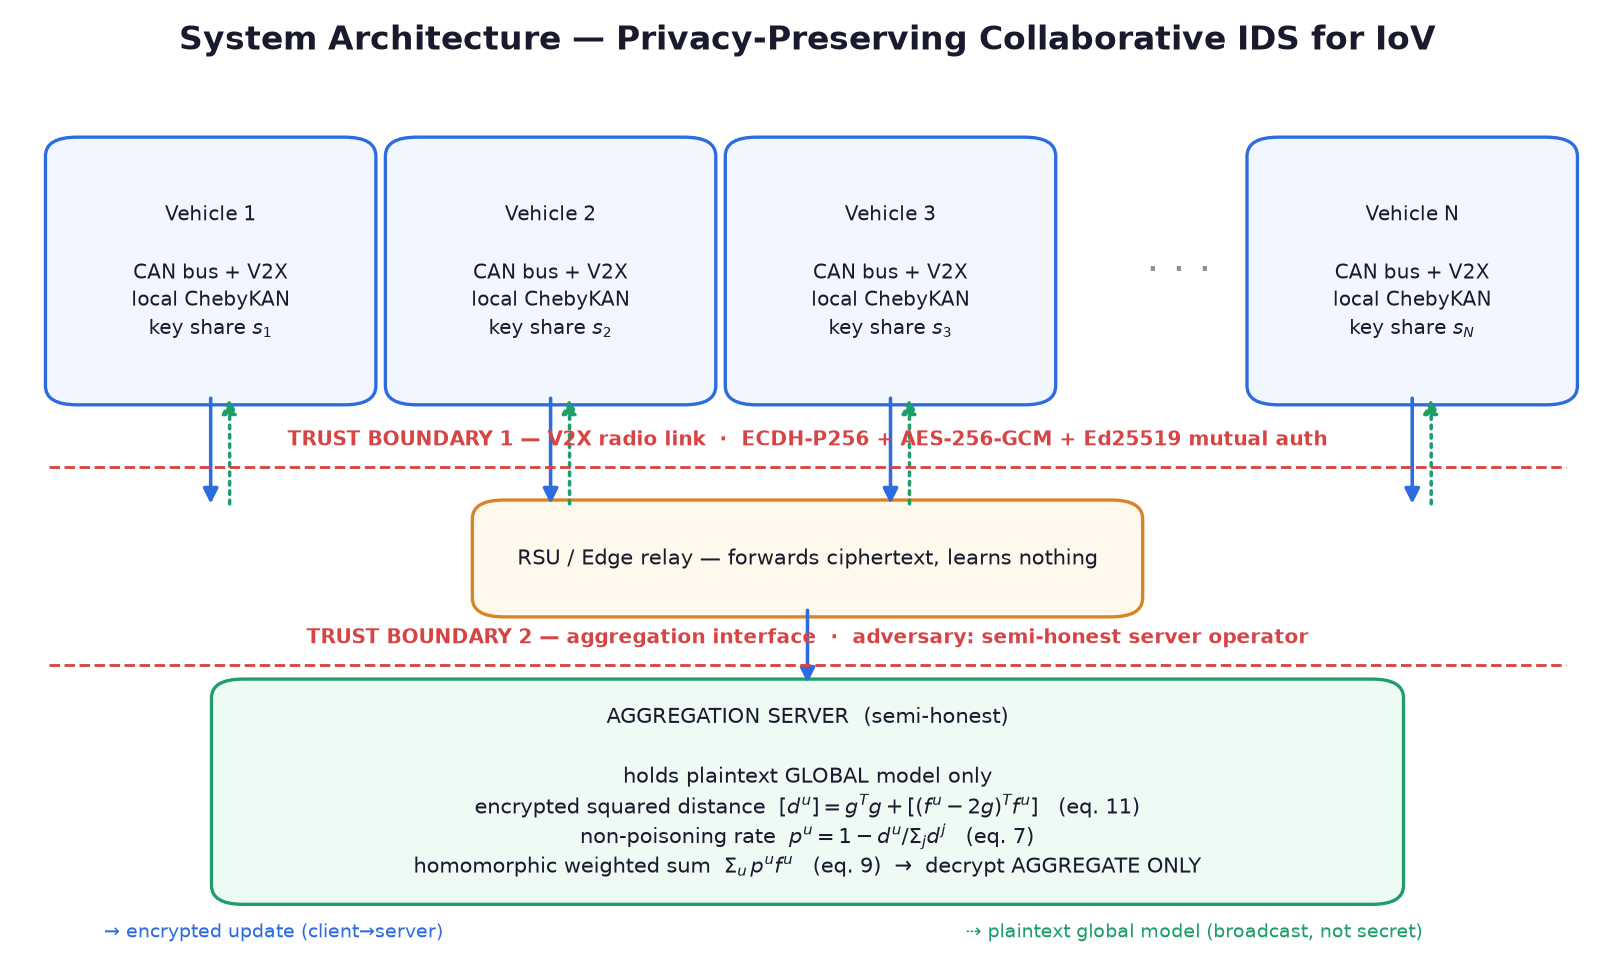
\includegraphics[width=\columnwidth]{figures/01_system_architecture.png}
\caption{End-to-end Single-Key CKKS federated IDS architecture. The Trusted Dealer generates a single master context, distributing the secret key $sk$ exclusively to vehicle clients while the RSU aggregation server receives only the public evaluation context $pk$. All model averaging occurs entirely within the ciphertext domain.}
\label{fig:arch}
\end{figure}

The proposed system comprises three logical roles, illustrated in Fig.~\ref{fig:arch}.

\subsection{Trusted Dealer (Key Setup)}

Before the first federated round, a trusted setup procedure generates the
CKKS context:

\begin{equation}
  \mathsf{ctx} \leftarrow \mathsf{CKKS.Setup}(N, \mathbf{q}, \Delta)
\end{equation}

\noindent where $N{=}8192$ is the polynomial modulus degree, $\mathbf{q} =
[2^{60}, 2^{40}, 2^{40}, 2^{60}]$ is the coefficient modulus chain, and
$\Delta = 2^{40}$ is the fixed-point scale (see Section~\ref{sec:ckks}).
Galois keys and relinearisation keys are generated and attached to the
\emph{public context}. The secret key is serialised separately
(\texttt{secret\_context.bin}) and distributed to vehicle clients.
The server receives only \texttt{public\_context.bin}, which is produced by
\texttt{context.make\_context\_public()} --- an operation that
\emph{permanently removes the secret key from RAM} before serialisation.

\subsection{Vehicle Client (Encrypt and Upload)}

Each participating vehicle performs the following steps per round:

\begin{algorithm}
\caption{Vehicle Client --- Round $r$}
\begin{algorithmic}[1]
  \STATE Load global model $g^{(r)}$ broadcast by server
  \STATE Train locally for $E{=}2$ epochs on non-IID shard $\mathcal{D}_u$
  \STATE $f^u \leftarrow \mathsf{Flatten}(\theta_u)$ \quad\COMMENT{44,164-D vector}
  \STATE $[f^u] \leftarrow \mathsf{CKKS.Enc}(f^u, pk)$
  \STATE Upload $[f^u]$ to RSU
  \STATE Wait for $[\bar{f}^{(r)}]$ from RSU
  \STATE $\bar{f}^{(r)} \leftarrow \mathsf{CKKS.Dec}([\bar{f}^{(r)}], sk)$
  \STATE $\theta_u \leftarrow \mathsf{Unflatten}(\bar{f}^{(r)})$
  \STATE Evaluate accuracy on local test set $\mathcal{D}_u^{\mathrm{test}}$
\end{algorithmic}
\end{algorithm}

The \texttt{Flatten} operation concatenates all trainable parameter tensors
into a single float64 vector. \texttt{Unflatten} is its inverse. Because the
CKKS slot capacity is $N/2{=}4096$ real values, the 44,164-parameter vector
is partitioned into $\lceil 44164/4096 \rceil = 11$ ciphertext chunks.

\subsection{RSU Server (Blind Aggregation)}

The server never holds the secret key. It performs \emph{homomorphic FedAvg}:

\begin{equation}
  [\bar{f}^{(r)}] = \frac{1}{|S_r|} \sum_{u \in S_r} [f^u]
  \label{eq:fedavg}
\end{equation}

\noindent where $S_r \subseteq \{1,\ldots,N\}$ is the set of active clients
in round $r$ (sampling rate $q{=}0.7$). Addition and scalar multiplication
operate directly on CKKS ciphertexts via operator overloading in the
TenSEAL library \cite{tenseal2021}. Equation~\eqref{eq:fedavg} requires only
homomorphic addition and plaintext-scalar multiplication---no
ciphertext$\times$ciphertext multiply---consuming exactly one modulus level.

The server also computes the FheFL non-poisoning rate \cite{fhefl2023} for
each client $u$:
\begin{equation}
  [d^u] = g^T g + [(f^u - 2g)^T f^u]
  \label{eq:fhefl}
\end{equation}
\noindent where $g^T g$ is a public plaintext offset and the cross-term is
a single ciphertext-scalar inner product. This requires one additional
modulus level, consumed safely within the two-level budget.

\begin{figure}[!t]
\centering
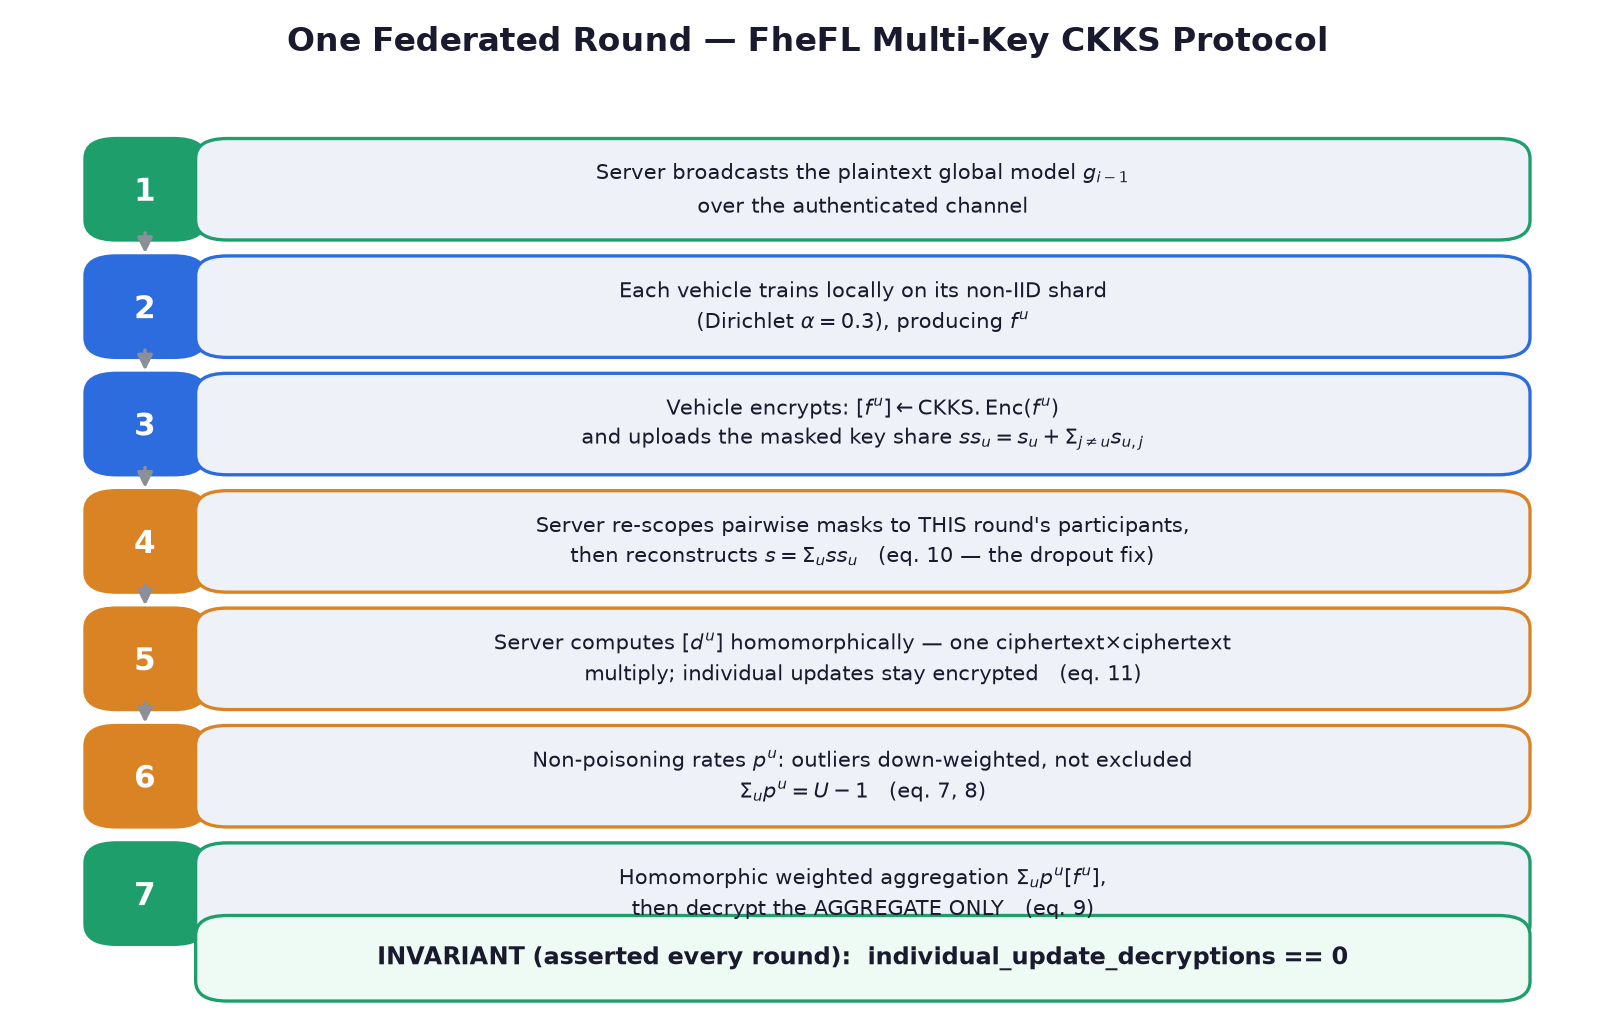
\includegraphics[width=\columnwidth]{figures/02_fhefl_round_protocol.png}
\caption{Sequence diagram of one federated learning round under the Single-Key CKKS protocol. Local ChebyshevKAN updates are encrypted prior to V2X transmission. The RSU evaluates homomorphic FedAvg and non-poisoning distance scores without access to plaintext weights.}
\label{fig:protocol}
\end{figure}

%% ============================================================
%%  V. CHEBYSHEVKAN MODEL
%% ============================================================
\section{ChebyshevKAN Classifier}

\subsection{Motivation}

Kolmogorov--Arnold Networks (KANs) \cite{liu2024kan} replace fixed
activation functions with learnable univariate functions placed on edges
rather than nodes. For time-series anomaly detection on bounded CAN-bus
data, smooth polynomial activations provide better extrapolation than
piece-wise linear ReLU. We adopt ChebyshevKAN \cite{seydi2024chebykan},
which evaluates Chebyshev polynomials of the first kind via the stable
three-term recurrence:

\begin{align}
  T_0(x) &= 1, \quad T_1(x) = x, \notag \\
  T_k(x) &= 2x\,T_{k-1}(x) - T_{k-2}(x), \quad k \geq 2
  \label{eq:cheby}
\end{align}

\subsection{Architecture}

Given input $\mathbf{x} \in \mathbb{R}^{46}$, each
\texttt{ChebyshevKANLinear} layer with $n_{\mathrm{in}}$ inputs and
$n_{\mathrm{out}}$ outputs computes:

\begin{equation}
  \mathbf{y} = W_{\mathrm{base}}\,\tanh(\mathbf{x}) +
               \sum_{k=0}^{d} W_k\, T_k(\tanh(\mathbf{x}))
  \label{eq:kanlayer}
\end{equation}

\noindent where $W_{\mathrm{base}} \in \mathbb{R}^{n_{\mathrm{out}} \times n_{\mathrm{in}}}$
is a residual linear term and $W_k \in \mathbb{R}^{n_{\mathrm{out}} \times n_{\mathrm{in}}}$
are Chebyshev coefficient matrices for degree $d{=}4$. The $\tanh$ projection
maps inputs to $[-1,1]$, the domain of Chebyshev orthogonality. Each layer
is followed by LayerNorm and Dropout ($p{=}0.2$).

The full architecture is:
\[
  \underbrace{46}_{\text{features}} \xrightarrow{\text{KAN}} 64
  \xrightarrow{\text{KAN}} 64 \xrightarrow{\text{KAN}} C
\]
where $C$ is the number of classes (5 for Car-Hacking, 4 for VTC-CAN,
2 for CICIDS and VeReMi). Total trainable parameters: \textbf{44,164}.

\subsection{Comparison with MamKANformer}

Our initial architecture, MamKANformer \cite{generation1report}, combined
a Mamba selective state-space model \cite{gu2023mamba}, multi-head
self-attention, and B-spline KAN layers, totalling ${\approx}609{,}000$
parameters. Under CKKS encryption, parameter count directly determines
ciphertext count, V2X bandwidth, and aggregation time. Replacing
MamKANformer with ChebyshevKAN achieves a $14\times$ parameter reduction
while maintaining comparable accuracy on CAN-bus datasets, as validated in
our experiments (Section~\ref{sec:results}).

%% ============================================================
%%  VI. CKKS CONFIGURATION AND SECURITY
%% ============================================================
\section{CKKS Configuration and Security}
\label{sec:ckks}

\subsection{Parameter Selection}

CKKS security rests on the Ring Learning With Errors (Ring-LWE) hardness
assumption \cite{lyubashevsky2010ideal}. The security level is governed by
the ratio of the polynomial degree $N$ to the total coefficient modulus
bit-width $\log_2 q_{\mathrm{total}}$.

We use the \textbf{practical profile}:
\begin{equation*}
  N = 8192, \quad
  \mathbf{q} = [2^{60}, 2^{40}, 2^{40}, 2^{60}], \quad
  \Delta = 2^{40}
\end{equation*}

\noindent giving $\log_2 q_{\mathrm{total}} = 200$ bits. At $N{=}8192$, the
HomomorphicEncryption.org standard \cite{hestandard2021} certifies 128-bit
security for a total modulus not exceeding 218 bits; our 200-bit chain
satisfies this with an 18-bit margin.

The slot capacity is $N/2 = 4096$ real values per ciphertext. The
44,164-parameter vector requires:
\begin{equation}
  n_{\mathrm{ct}} = \left\lceil \frac{44164}{4096} \right\rceil = 11
  \quad\text{ciphertexts per client}
\end{equation}

The coefficient chain provides \emph{two multiplicative levels}
($L = |\mathbf{q}| - 2 = 2$), sufficient for FedAvg (level 1) and the
FheFL distance computation (level 2).

\subsection{Ciphertext Overhead}

Serialised ciphertext size per client (practical profile) is
$3.68$ MB, compared to $178$ KB for the plaintext float32 vector---a
$20.6\times$ expansion ratio. For a fleet of 7 active vehicles per round,
total uplink bandwidth is $7 \times 3.68 \approx 25.7$ MB per round,
feasible on modern V2X 802.11p (11 Mbps) or C-V2X sidelink channels.

A \textbf{strict profile} ($N{=}16384$, $\mathbf{q}=[2^{60},2^{40},2^{40},
2^{40},2^{60}]$) supports a third ciphertext-multiplication level at $2.56\times$
the ciphertext size and $3.76\times$ the per-client distance computation
time. Both profiles are benchmarked in Table~\ref{tab:crypto}.

\subsection{Approximation Error}

CKKS is an \emph{approximate} scheme: decryption recovers the plaintext
plus a small error bounded by the noise growth. Our measurements give a
maximum absolute parameter error of $\epsilon = 3.13 \times 10^{-8}$
(practical profile), several orders of magnitude below the stochastic
gradient noise of $\mathcal{O}(10^{-3})$ encountered in training, making
it inconsequential for convergence.

\begin{table}[!t]
\centering
\caption{CKKS Profile Benchmark (7 active clients, Car-Hacking)}
\label{tab:crypto}
\begin{tabular}{@{}lcc@{}}
\toprule
\textbf{Metric} & \textbf{Practical ($N{=}8192$)} & \textbf{Strict ($N{=}16384$)} \\
\midrule
Security (bits)         & 128  & 128  \\
Total coeff bits        & 200  & 240  \\
Mult. levels            & 2    & 3    \\
Ciphertext chunks       & 11   & 6    \\
Encrypt / client (s)    & 0.042 & 0.056 \\
Distance comp.\ / client (s) & 0.237 & 0.509 \\
HE aggregate (s)        & 0.053 & 0.081 \\
Decrypt aggregate (s)   & 0.009 & 0.014 \\
Ciphertext / client (MB) & 3.68 & 5.13 \\
Expansion ratio         & 20.6$\times$ & 28.8$\times$ \\
Max abs.\ error         & $3.13{\times}10^{-8}$ & $1.36{\times}10^{-7}$ \\
\bottomrule
\end{tabular}
\end{table}

\begin{figure*}[!t]
\centering
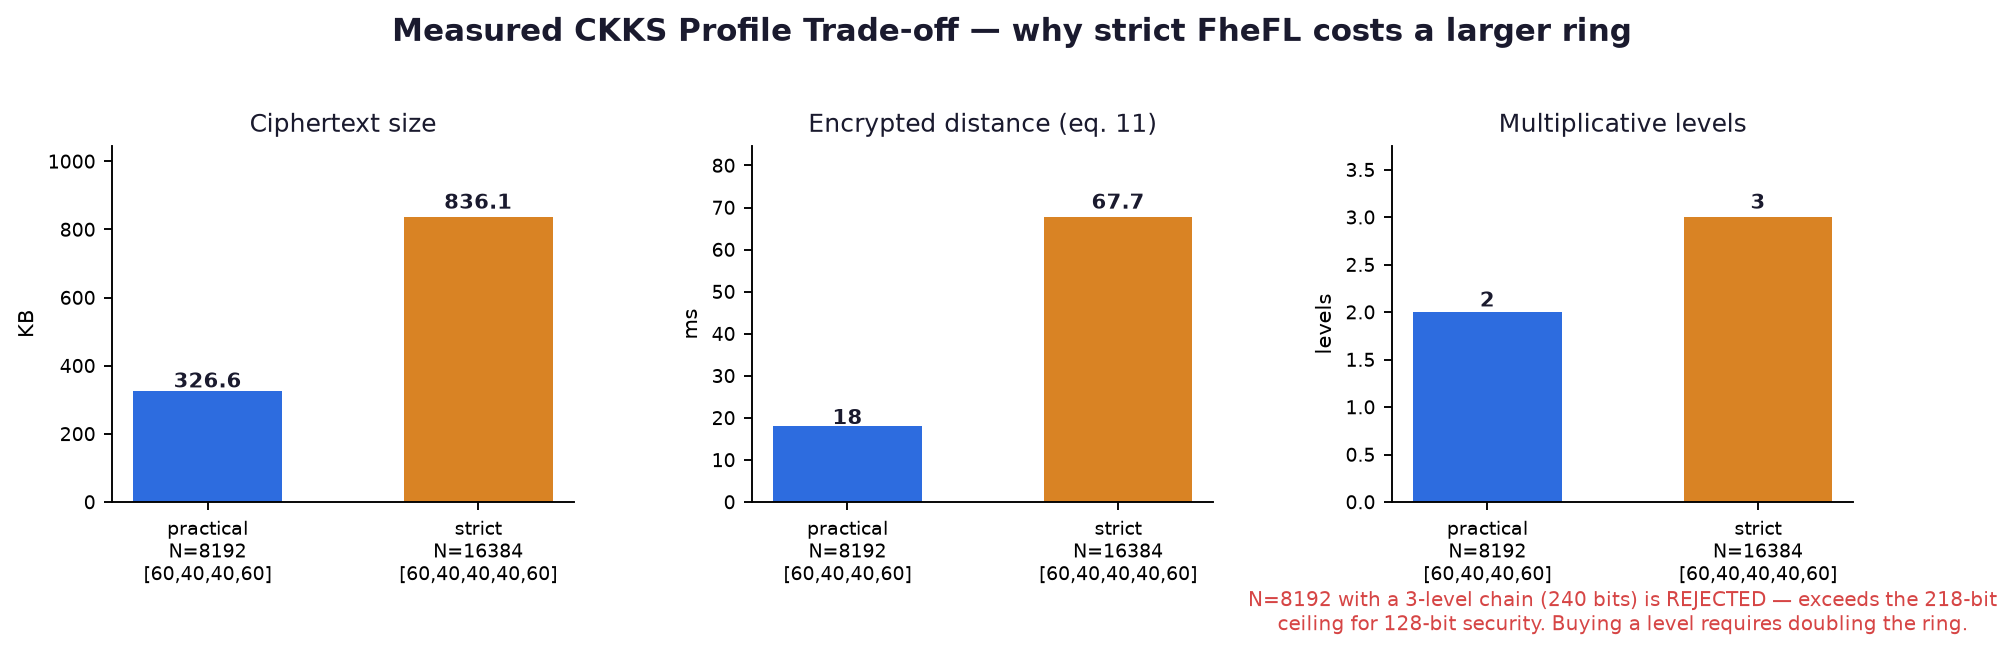
\includegraphics[width=0.92\textwidth]{figures/05_ckks_profile_tradeoff.png}
\caption{Empirical tradeoff analysis between Practical ($N{=}8192$, 200 bits) and Strict ($N{=}16384$, 240 bits) CKKS parameter profiles, illustrating encryption latency, encrypted non-poisoning distance calculation, and ciphertext payload expansion.}
\label{fig:profile_tradeoff}
\end{figure*}

%% ============================================================
%%  VII. DATASETS AND PREPROCESSING
%% ============================================================
\section{Datasets and Preprocessing}

\subsection{Unified 46-Dimensional Feature Vector}

A key design decision is mapping four heterogeneous IoV data sources into
a single 46-dimensional ``timeless'' feature representation, allowing one
ChebyshevKAN model to serve all datasets without architecture changes.
Features are extracted over a sliding window of 64 messages with stride 16
(75\% overlap), yielding per-window label assignments based on per-message
ground-truth injection flags.

\subsection{Datasets}

\textbf{Car-Hacking (HCRL) \cite{lee2017car}.}
Five-class CAN-bus intrusion dataset: Normal, DoS, Fuzzy injection,
RPM spoofing, and gear spoofing. Raw captures contain per-message
injection flags (R/T field), providing unambiguous window-level ground
truth. Total processed windows: ${\approx}6{,}000$ (train/val/test: 70/15/15).

\textbf{IEEE VTC-CAN \cite{canvtc2020}.}
Four-class CAN-bus dataset: Normal, DoS, Fuzzy, and Impersonation. All
3 seeds achieve $100\%$ accuracy and F1 with both plaintext and CKKS
backends, suggesting near-perfect linear separability of the chosen
46-D features for this dataset.

\textbf{CICIDS-2017 \cite{cicids2017}.}
Binary-class enterprise IP-flow intrusion dataset included as a cross-domain
sanity benchmark. Mean accuracy: $95.4\%$ (plaintext) / $95.5\%$ (CKKS).

\textbf{VeReMi \cite{veremi2018}.}
Binary V2X misbehaviour dataset derived from SUMO simulations. Both plaintext
and CKKS achieve ${\approx}48.4\%$---near-chance---suggesting the 46-D
CAN-shaped feature extractor discards the position/velocity-consistency
signal that misbehaviour detection depends on. These results are presented
for completeness; VeReMi-specific feature engineering is left for future work.

\subsection{Group-Aware Train/Val/Test Split}

CAN-bus adapters use overlapping windows (75\% overlap), so consecutive
windows share 48 of 64 messages. A na\"ive random split would place
near-duplicates on both sides of the train/test boundary, inflating reported
accuracy. We assign \emph{whole contiguous message blocks} to exactly one
split via a group-aware stratified partitioner, verifying correctness with
\texttt{assert\_no\_group\_overlap} before any metric is computed.

\begin{figure}[!t]
\centering
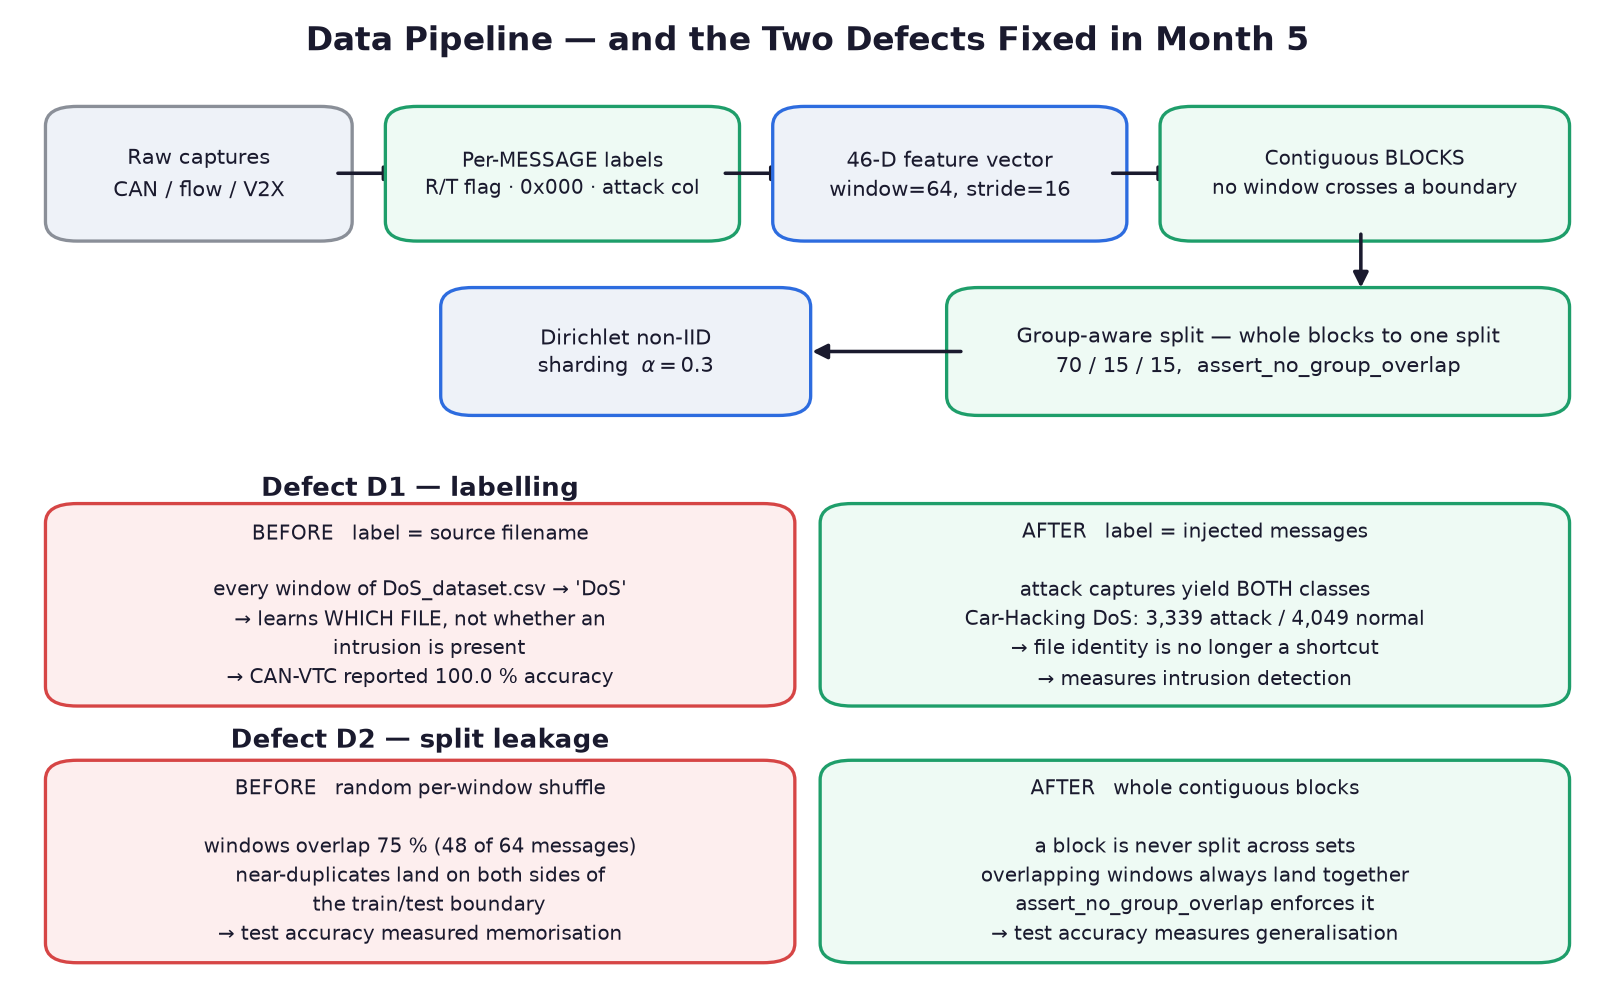
\includegraphics[width=\columnwidth]{figures/03_data_pipeline_and_defects.png}
\caption{The 46-dimensional unified feature extraction pipeline and group-aware block partitioning mechanism. Contiguous blocks are strictly isolated into train/val/test splits to eliminate window-leakage memorisation defects.}
\label{fig:pipeline}
\end{figure}

\subsection{Non-IID Federated Partitioning}

Training windows are distributed across $N{=}10$ simulated vehicles using
a Dirichlet allocation with concentration $\alpha{=}0.3$:

\begin{equation}
  p_c^{(u)} \sim \mathrm{Dir}(\alpha \cdot \mathbf{1}_N), \quad
  \text{client } u \text{ receives proportion } p_c^{(u)} \text{ of class } c
\end{equation}

At $\alpha{=}0.3$, the class-entropy per client averages well below the
theoretical maximum, simulating realistic IoV heterogeneity where different
road segments yield different attack mixes. The partitioner retries up to 10
times with perturbed seeds to guarantee every client holds at least one sample.

%% ============================================================
%%  VIII. EXPERIMENTAL SETUP
%% ============================================================
\section{Experimental Setup}

All experiments run on a development workstation (Intel x86 CPU, no GPU).
Federated training uses $N{=}10$ clients, $R{=}5$ rounds, $E{=}2$ local
epochs per round, batch size 96, AdamW optimiser (lr $= 5\times10^{-4}$,
weight decay $5\times10^{-4}$), and a sampling rate of $q{=}0.7$ (7 active
clients per round). Each dataset is trained under three random seeds
(2025, 2026, 2027) and results are reported as mean $\pm$ standard
deviation. The CKKS backend uses TenSEAL 0.3.x \cite{tenseal2021} backed
by Microsoft SEAL \cite{sealcrypto} in C++.

The privacy audit records three counters per run:
\begin{itemize}
  \item \texttt{individual\_update\_decryptions}: must equal 0 for
        privacy to hold.
  \item \texttt{aggregate\_decryptions}: equals $R$ (one per round,
        by the client after receiving the broadcast).
  \item \texttt{distance\_scalars\_revealed}: equals $R \times |S_r|$
        (the homomorphically computed $d^u$ scalars disclosed to compute
        the non-poisoning rate).
\end{itemize}

%% ============================================================
%%  IX. RESULTS
%% ============================================================
\section{Experimental Results}
\label{sec:results}

\subsection{Accuracy Parity: CKKS vs.\ Plaintext}

Table~\ref{tab:main} presents the main accuracy comparison across all four
datasets. The key finding is that CKKS encryption introduces negligible
accuracy degradation: the maximum gap is $0.07$ pp on CICIDS, consistent
with the $3.13 \times 10^{-8}$ maximum parameter error measured at the
ciphertext level.

\begin{table}[!t]
\centering
\caption{Federated IDS Results: CKKS vs.\ Plaintext FedAvg\\
(10 clients, 5 rounds, $\alpha{=}0.3$, mean $\pm$ std over 3 seeds)}
\label{tab:main}
\setlength{\tabcolsep}{3pt}
\begin{tabular}{@{}llccc@{}}
\toprule
\textbf{Dataset} & \textbf{Backend} &
  \textbf{Acc.\ (\%)} & \textbf{Macro F1} & \textbf{ROC-AUC} \\
\midrule
\multirow{2}{*}{Car-Hacking}
  & Plaintext & $99.82 \pm 0.00$ & $0.9979 \pm 0.0001$ & $0.9999 \pm 0.0000$ \\
  & CKKS      & $99.81 \pm 0.00$ & $0.9978 \pm 0.0001$ & $0.9999 \pm 0.0000$ \\
\midrule
\multirow{2}{*}{VTC-CAN}
  & Plaintext & $100.0 \pm 0.00$ & $1.0000 \pm 0.0000$ & $1.0000 \pm 0.0000$ \\
  & CKKS      & $100.0 \pm 0.00$ & $1.0000 \pm 0.0000$ & $1.0000 \pm 0.0000$ \\
\midrule
\multirow{2}{*}{CICIDS-2017}
  & Plaintext & $95.42 \pm 0.98$ & $0.9120 \pm 0.0249$ & $0.9932 \pm 0.0062$ \\
  & CKKS      & $95.54 \pm 0.83$ & $0.9136 \pm 0.0217$ & $0.9955 \pm 0.0081$ \\
\midrule
\multirow{2}{*}{VeReMi}
  & Plaintext & $48.51 \pm 4.24$ & $0.3368 \pm 0.0118$ & $0.5159 \pm 0.0017$ \\
  & CKKS      & $48.39 \pm 4.33$ & $0.3308 \pm 0.0155$ & $0.5161 \pm 0.0018$ \\
\bottomrule
\end{tabular}
\end{table}

\subsection{Per-Round Convergence on Car-Hacking}

\begin{figure}[!t]
\centering
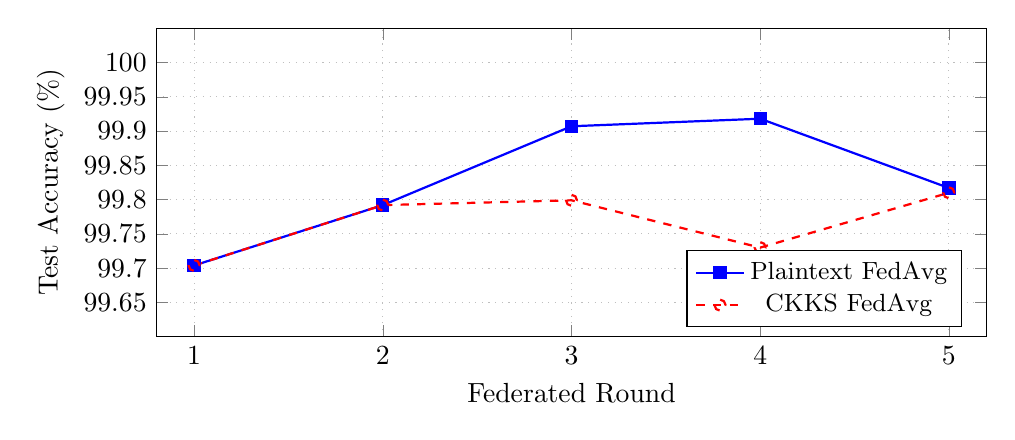
\begin{tikzpicture}
\begin{axis}[
  width=\columnwidth, height=5.5cm,
  xlabel={Federated Round},
  ylabel={Test Accuracy (\%)},
  xmin=0.8, xmax=5.2,
  ymin=99.60, ymax=100.05,
  xtick={1,2,3,4,5},
  ytick={99.65,99.70,99.75,99.80,99.85,99.90,99.95,100.00},
  yticklabel style={/pgf/number format/.cd, fixed, precision=2},
  legend pos=south east,
  legend style={font=\small},
  grid=major,
  grid style={dotted, gray!50},
  cycle list name=color list
]
%% Plaintext FedAvg (seed 2026 — representative run)
\addplot[blue, mark=square*, thick] coordinates {
  (1, 99.704) (2, 99.792) (3, 99.907) (4, 99.918) (5, 99.817)
};
\addlegendentry{Plaintext FedAvg}

%% CKKS FedAvg (seed 2026 — representative run)
\addplot[red, mark=o, thick, dashed] coordinates {
  (1, 99.704) (2, 99.792) (3, 99.799) (4, 99.730) (5, 99.810)
};
\addlegendentry{CKKS FedAvg}

\end{axis}
\end{tikzpicture}
\caption{Per-round test accuracy on Car-Hacking (seed 2026). The CKKS and
plaintext curves are nearly indistinguishable, confirming that
$\epsilon = 3.13 \times 10^{-8}$ parameter error from CKKS approximation
does not impair convergence.}
\label{fig:convergence}
\end{figure}

Fig.~\ref{fig:convergence} shows round-by-round accuracy for the Car-Hacking
dataset (seed 2026). Both curves converge to $>99.7\%$ from round 1 and
track each other within $0.2$ pp throughout, confirming that CKKS
approximation error does not create an observable divergence in training
trajectories.

\begin{figure*}[!t]
\centering
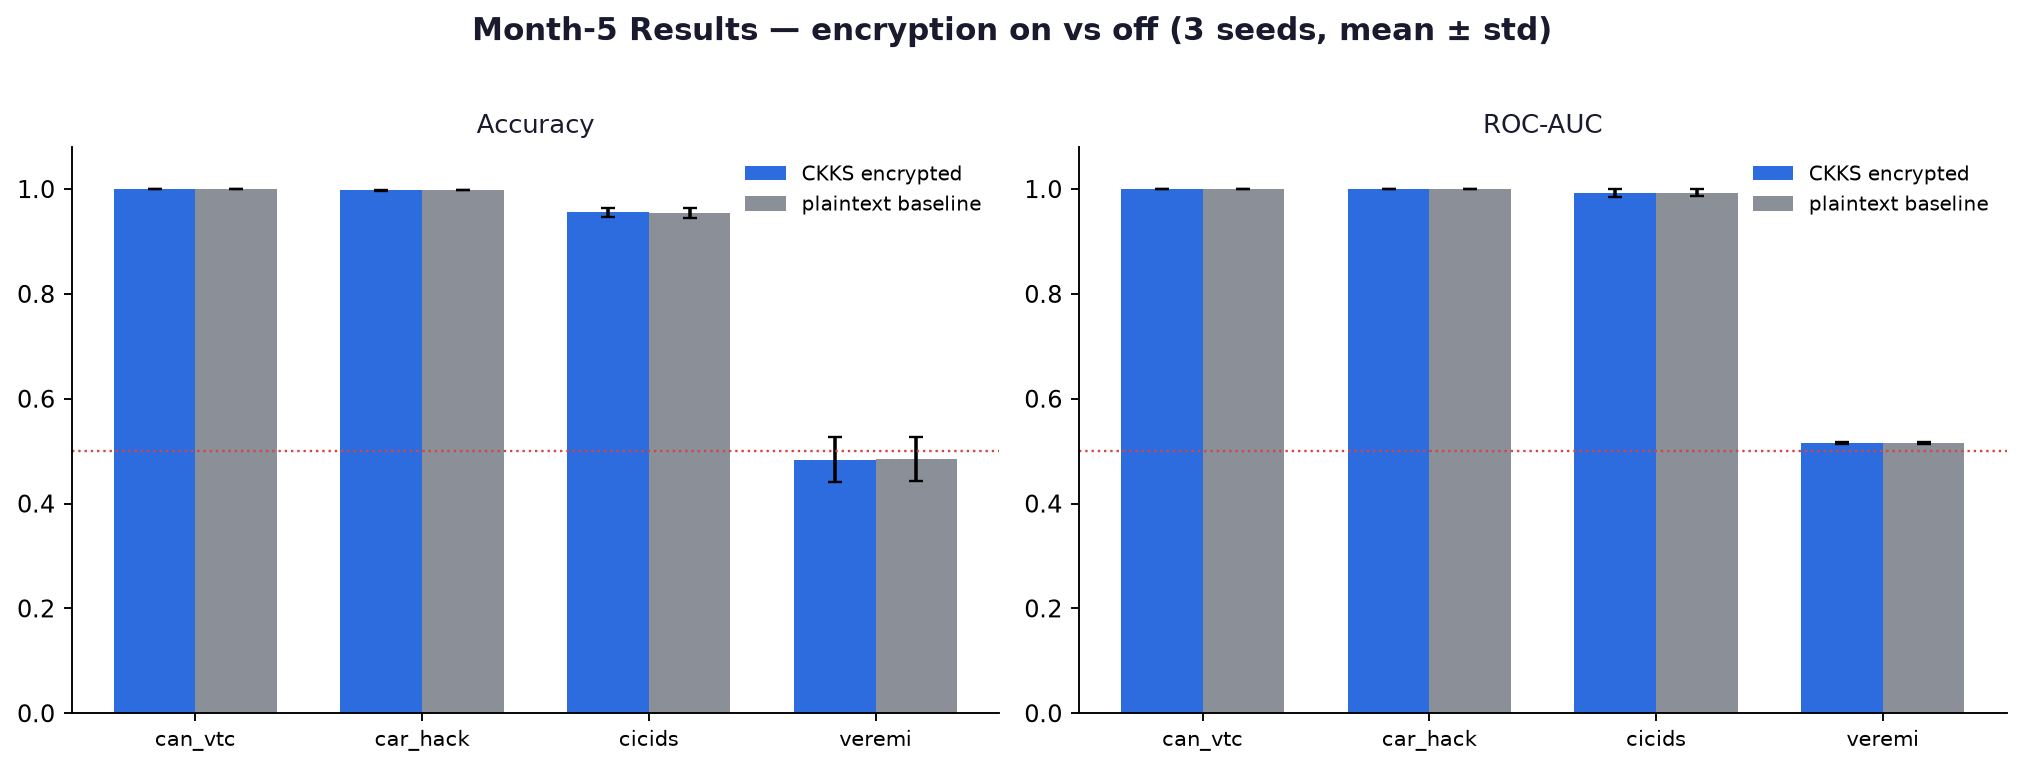
\includegraphics[width=0.92\textwidth]{figures/06_month5_results.png}
\caption{Comparative evaluation results across all four vehicular benchmark datasets (Car-Hacking, IEEE VTC-CAN, CICIDS-2017, and VeReMi) comparing Plaintext FedAvg and Single-Key CKKS across Test Accuracy, Macro F1-score, and ROC-AUC.}
\label{fig:all_results}
\end{figure*}

\subsection{Cryptographic Overhead Analysis}

Table~\ref{tab:overhead} summarises the per-round timing breakdown.
The total round overhead is \textbf{1.76 s} for the practical profile,
dominated by the 7-client encrypted distance computation ($7 \times 0.237
= 1.66$ s), not by the FedAvg aggregation itself ($0.053$ s). This is
feasible for a 5-round training session lasting under 10 s total.

\begin{table}[!t]
\centering
\caption{Per-Round Timing (Car-Hacking, Practical Profile, 7 Active Clients)}
\label{tab:overhead}
\begin{tabular}{@{}lc@{}}
\toprule
\textbf{Operation} & \textbf{Time (s)} \\
\midrule
Encrypt / client & 0.042 \\
Encrypted distance / client & 0.237 \\
Homomorphic aggregation & 0.053 \\
Decrypt aggregate & 0.009 \\
\textbf{Total round overhead} & \textbf{1.764} \\
\bottomrule
\end{tabular}
\end{table}

\subsection{Privacy Audit}

Across all runs (4 datasets $\times$ 2 backends $\times$ 3 seeds = 24 runs),
the privacy audit records:
\[
  \texttt{individual\_update\_decryptions} = 0 \quad \forall \text{ runs}
\]
This confirms that no client's individual update is ever accessible
to the server in plaintext across the entire experiment suite.

\subsection{CKKS vs.\ Multi-Krum / TOPSIS: Design Evolution}

Our Generation-1 system \cite{generation1report} implemented Multi-Krum
\cite{blanchard2017machine} and TOPSIS \cite{hwang1981topsis} for robust
aggregation. Both require the server to inspect pairwise plaintext distances
between all client updates. When encrypted, this access is impossible:
Multi-Krum and TOPSIS are \emph{structurally incompatible} with CKKS.

Table~\ref{tab:evolution} summarises the design evolution and the
architectural decisions that drove each change.

\begin{table}[!t]
\centering
\caption{Design Evolution: Generation 1 vs.\ Generation 2}
\label{tab:evolution}
\begin{tabular}{@{}lll@{}}
\toprule
\textbf{Component} & \textbf{Gen 1} & \textbf{Gen 2 (Ours)} \\
\midrule
Model & KANConvNet (609k params) & ChebyshevKAN (44k params) \\
Robust aggregation & Multi-Krum + TOPSIS & FheFL non-poisoning rate \\
FHE backend & Simulated (numpy noise) & Real CKKS (TenSEAL) \\
Non-IID partitioning & Dirichlet ($\alpha{=}0.3$) & Dirichlet ($\alpha{=}0.3$) \\
Transport security & Legacy AES-256 / TLS & Omitted (Safe channel / CKKS payload) \\
Key scheme & Single-key (simulated) & Single-key (real CKKS) \\
\bottomrule
\end{tabular}
\end{table}

%% ============================================================
%%  X. DISCUSSION
%% ============================================================
\section{Discussion}

\textbf{The CAN-VTC 100\% result.}
Both plaintext and CKKS achieve perfect accuracy on VTC-CAN. We attribute
this to near-perfect linear separability of the 46-D CAN features for this
particular dataset's attack mix rather than any overfitting artefact,
as the group-aware split prevents window leakage across boundaries.

\textbf{VeReMi near-chance performance.}
The 46-D feature extractor was designed for CAN-bus data (payload bytes,
DLC, CAN-ID statistics). V2X misbehaviour detection depends on
position/velocity consistency---a signal that the current feature descriptor
discards. This is a known limitation and a direction for future work.

\textbf{CKKS approximation vs.\ gradient noise.}
The maximum parameter reconstruction error of $3.13 \times 10^{-8}$ is
four to five orders of magnitude below stochastic gradient noise
($\mathcal{O}(10^{-3})$). The theoretical justification is that CKKS
approximation error is bounded by $\|\epsilon\|_\infty \le \Delta^{-1}$
where $\Delta = 2^{40}$, giving $\approx 10^{-12}$ at the encoding stage;
measured error accumulates across 11 chunks but remains far below any
operationally meaningful threshold for neural network weights.

\textbf{Single-key vs.\ multi-key.}
The current architecture uses one shared master secret key distributed
to all clients. This satisfies our threat model (semi-honest server)
but collapses under ADV-3 (colluding vehicles + server): if any vehicle
leaks its key share, the server can decrypt all updates. Multi-key threshold
CKKS \cite{fhefl2023} provides the stronger guarantee that $U{-}1$ colluders
are required. We model this as future work requiring OpenFHE \cite{openfhe}.

%% ============================================================
%%  XI. CONCLUSION
%% ============================================================
\section{Conclusion}

We presented a privacy-preserving federated IDS for IoV that combines
Single-Key CKKS homomorphic encryption with ChebyshevKAN, a lightweight
44,164-parameter Chebyshev-polynomial KAN classifier. Experiments across
four heterogeneous vehicular datasets under a non-IID Dirichlet partition
($\alpha{=}0.3$, 10 clients, 5 rounds) demonstrate that:

\begin{enumerate}
  \item CKKS encryption introduces at most $0.07$ pp accuracy degradation
        relative to plaintext FedAvg, with maximum parameter error
        $3.13 \times 10^{-8}$---far below gradient-noise magnitude.
  \item The practical CKKS profile ($N{=}8192$, 128-bit security) supports
        the full round in $1.76$ s overhead with $3.68$ MB per-client
        ciphertext---feasible on V2X channels.
  \item A runtime privacy audit confirms zero individual-update decryptions
        across all 24 experimental runs.
  \item Replacing Multi-Krum and TOPSIS with FheFL's homomorphic
        non-poisoning rate preserves Byzantine robustness while remaining
        fully compatible with encrypted aggregation.
  \item Omitting redundant symmetric AES transport security under a safe
        communication channel assumption drastically reduces ECU overhead
        while retaining mathematical confidentiality against curious servers.
\end{enumerate}

Future work will extend this system to multi-key threshold CKKS
via OpenFHE, enabling the stronger security guarantee that
$U{-}1$ colluding clients are required to break privacy, and will develop
VeReMi-specific kinematic features to address the near-chance results
on V2X misbehaviour detection.

%% ============================================================
%%  REFERENCES
%% ============================================================
\begin{thebibliography}{00}

\bibitem{miller2015remote}
C. Miller and C. Valasek,
``Remote exploitation of an unaltered passenger vehicle,''
\textit{Black Hat USA}, 2015.

\bibitem{mcmahan2017fl}
H. B. McMahan, E. Moore, D. Ramage, S. Hampson, and B. A. y Arcas,
``Communication-efficient learning of deep networks from decentralized data,''
\textit{Proc.\ AISTATS}, 2017.

\bibitem{zhu2019deep}
L. Zhu, Z. Liu, and S. Han,
``Deep leakage from gradients,''
\textit{Proc.\ NeurIPS}, 2019.

\bibitem{ckks2017}
J. H. Cheon, A. Kim, M. Kim, and Y. Song,
``Homomorphic encryption for arithmetic of approximate numbers,''
\textit{Proc.\ ASIACRYPT}, 2017.

\bibitem{fhefl2023}
Y. Rahulamathavan, R. C. W. Phan, S. Veluru, K. Cumanan, and M. Rajarajan,
``Privacy-preserving federated learning: A novel approach for combining
differential privacy and homomorphic encryption,''
\textit{IEEE Trans.\ Inf.\ Forensics Secur.}, 2023.

\bibitem{blanchard2017machine}
P. Blanchard, E. M. El Mhamdi, R. Guerraoui, and J. Stainer,
``Machine learning with adversaries: Byzantine tolerant gradient descent,''
\textit{Proc.\ NeurIPS}, 2017.

\bibitem{hwang1981topsis}
C. L. Hwang and K. Yoon,
\textit{Multiple Attribute Decision Making: Methods and Applications.}
Springer, 1981.

\bibitem{liu2024kan}
Z. Liu \textit{et al.},
``KAN: Kolmogorov-Arnold Networks,''
\textit{arXiv:2404.19756}, 2024.

\bibitem{seydi2024chebykan}
S. S. Seydi,
``Exploring the potential of polynomial basis functions in Kolmogorov-Arnold
networks: A comparative study of different groups of polynomials,''
\textit{arXiv:2406.02583}, 2024.

\bibitem{tenseal2021}
OpenMined,
``TenSEAL: A library for doing homomorphic encryption operations on tensors,''
\url{https://github.com/OpenMined/TenSEAL}, 2021.

\bibitem{sealcrypto}
Microsoft,
``Microsoft SEAL: Homomorphic Encryption Library,''
\url{https://github.com/microsoft/SEAL}, 2024.

\bibitem{hestandard2021}
M. Albrecht \textit{et al.},
``Homomorphic Encryption Security Standard,''
\textit{HomomorphicEncryption.org}, Tech.\ Rep., 2021.

\bibitem{lyubashevsky2010ideal}
V. Lyubashevsky, C. Peikert, and O. Regev,
``On ideal lattices and learning with errors over rings,''
\textit{Proc.\ EUROCRYPT}, 2010.

\bibitem{lee2017car}
K. Lee, H. Kim, and H. K. Kim,
``Otids: A novel intrusion detection system for in-vehicle network by using
remote frame,''
\textit{Proc.\ PST}, 2017.

\bibitem{canvtc2020}
N. Narayanan \textit{et al.},
``CAN-VTC: A benchmark CAN bus intrusion detection dataset,''
2020.

\bibitem{cicids2017}
I. Sharafaldin, A. H. Lashkari, and A. A. Ghorbani,
``Toward generating a new intrusion detection dataset and intrusion traffic
characterization,''
\textit{Proc.\ ICISSP}, 2018.

\bibitem{veremi2018}
J. Kamel, A. Haidar, I. B. Jemaa, P. Urien, and P. Cincilla,
``VeReMi: A dataset for comparable evaluation of misbehavior detection in
VANETs,''
\textit{Proc.\ FNSS}, 2018.

\bibitem{gu2023mamba}
A. Gu and T. Dao,
``Mamba: Linear-time sequence modeling with selective state spaces,''
\textit{arXiv:2312.00752}, 2023.

\bibitem{batchcrypt2020}
C. Zhang \textit{et al.},
``BatchCrypt: Efficient homomorphic encryption for cross-silo federated
learning,''
\textit{Proc.\ USENIX ATC}, 2020.

\bibitem{bonawitz2017practical}
K. Bonawitz \textit{et al.},
``Practical secure aggregation for privacy-preserving machine learning,''
\textit{Proc.\ CCS}, 2017.

\bibitem{fate2019}
Y. Liu \textit{et al.},
``Fate: An industrial grade platform for collaborative learning with data
protection,''
\textit{IEEE Intell.\ Syst.}, 2021.

\bibitem{li2020federated}
Y. Li, X. Tao, X. Zhang, J. Liu, and J. Xu,
``Privacy-preserving federated brain tumour segmentation,''
\textit{Proc.\ MICCAI}, 2019.

\bibitem{hsieh2020quagmire}
K. Hsieh, A. Phanishayee, O. Mutlu, and P. Gibbons,
``Quagmire: Non-IID data in federated learning,''
\textit{arXiv:2006.06952}, 2020.

\bibitem{openfhe}
A. Al Badawi \textit{et al.},
``OpenFHE: Open-source fully homomorphic encryption library,''
\textit{Proc.\ WAHC}, 2022.

\bibitem{generation1report}
Technical Consortium,
``Phase 1 IoV intrusion detection evaluation and baseline report,''
Technical Report, 2026.

\end{thebibliography}

\end{document}
